\documentclass[tikz,border=14pt]{standalone}
\usepackage{amsmath,amssymb}
\usetikzlibrary{arrows.meta,decorations.markings,calc,bending}

\definecolor{inkDark}{HTML}{1E293B}
\definecolor{pathBlue}{HTML}{005A9C}
\definecolor{velRed}{HTML}{C0392B}
\definecolor{mapTeal}{HTML}{0E6251}
\definecolor{axisSlate}{HTML}{334155}

\begin{document}
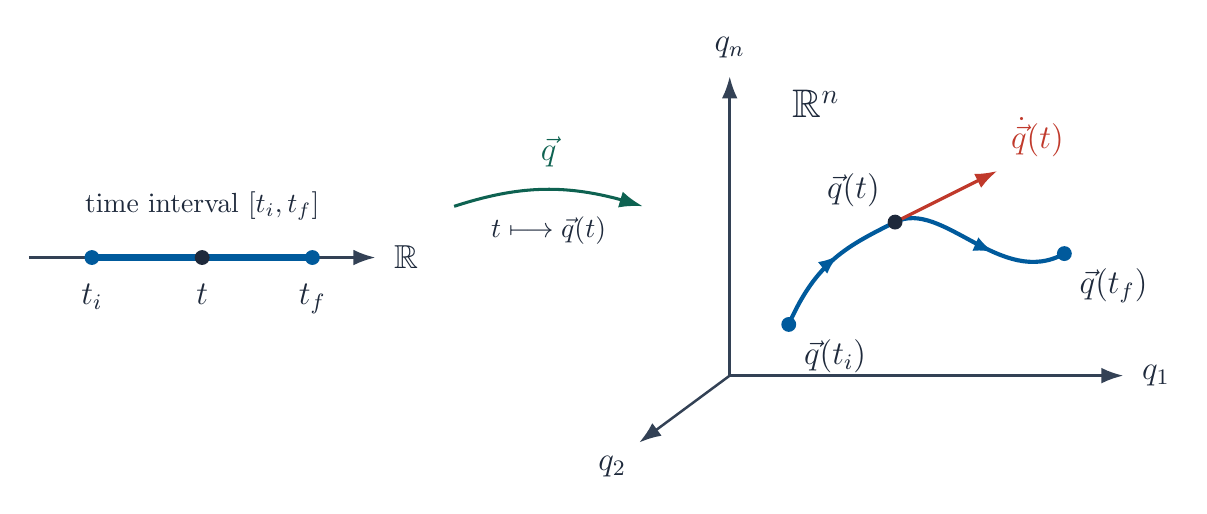
\begin{tikzpicture}[
    >=Latex,
    every node/.style={font=\large, text=inkDark},
    axis/.style={-{Latex[length=2.8mm,width=2.0mm]}, line width=0.9pt, draw=axisSlate},
    maparrow/.style={-{Latex[length=3.0mm,width=2.1mm]}, line width=1.1pt, draw=mapTeal},
    traj/.style={
        line width=1.5pt,
        draw=pathBlue,
        postaction={decorate},
        decoration={
            markings,
            mark=at position 0.26 with {\arrow{Latex[length=2.6mm,width=1.9mm]}},
            mark=at position 0.78 with {\arrow{Latex[length=2.6mm,width=1.9mm]}}
        }
    },
    vel/.style={-{Latex[length=2.8mm,width=2.0mm]}, line width=1.2pt, draw=velRed},
    pt/.style={circle, fill=inkDark, inner sep=1.9pt}
]

    % --- Left: Time domain [t_i, t_f] \subset \mathbb{R} ---
    \draw[axis] (-0.5, 0.4) -- (3.9, 0.4) node[right=3pt] {$\mathbb{R}$};
    \draw[line width=2.6pt, draw=pathBlue] (0.3, 0.4) -- (3.1, 0.4);

    % Points on time interval
    \node[pt, fill=pathBlue] (ti) at (0.3, 0.4) {};
    \node[pt, fill=inkDark]  (tm) at (1.7, 0.4) {};
    \node[pt, fill=pathBlue] (tf) at (3.1, 0.4) {};

    \node[below=6pt] at (ti) {$t_i$};
    \node[below=6pt] at (tm) {$t$};
    \node[below=6pt] at (tf) {$t_f$};
    \node[above=10pt, font=\normalsize, text=inkDark] at (1.7, 0.4) {time interval $[t_i, t_f]$};

    % --- Middle: Mapping arrow \vec{q} ---
    \draw[maparrow] (4.9, 1.05) to[bend left=18]
        node[above=4pt, text=mapTeal] {$\vec{q}$}
        node[below=6pt, font=\normalsize, text=inkDark] {$t \longmapsto \vec{q}(t)$}
        (7.3, 1.05);

    % --- Right: Configuration space \mathbb{R}^n ---
    \begin{scope}[shift={(8.4, -1.1)}]
        % Coordinate axes of \mathbb{R}^n
        \draw[axis] (0, 0) -- (5.0, 0) node[right=3pt] {$q_1$};
        \draw[axis] (0, 0) -- (0, 3.8) node[above=3pt] {$q_n$};
        \draw[axis] (0, 0) -- (-1.15, -0.85) node[below left=1pt] {$q_2$};
        \node[font=\Large, text=inkDark] at (1.1, 3.45) {$\mathbb{R}^n$};

        % Trajectory curve \vec{q}(t): exact cubic Bezier segments with matched tangent at Qm
        \coordinate (Qi) at (0.75, 0.65);
        \coordinate (Qm) at (2.10, 1.95);
        \coordinate (Qf) at (4.25, 1.55);

        \draw[traj] (Qi) .. controls (1.10, 1.45) and (1.50, 1.65) .. (Qm)
                         .. controls (2.70, 2.25) and (3.45, 1.10) .. (Qf);

        % Tangent velocity vector \dot{\vec{q}}(t) at \vec{q}(t) along exact tangent direction (2, 1)
        \draw[vel] (Qm) -- ++(1.30, 0.65) node[above right=1pt, text=velRed] {$\dot{\vec{q}}(t)$};

        % Endpoints and intermediate point on the curve
        \node[pt, fill=pathBlue] at (Qi) {};
        \node[pt, fill=inkDark]  at (Qm) {};
        \node[pt, fill=pathBlue] at (Qf) {};

        \node[below right=2pt] at (Qi) {$\vec{q}(t_i)$};
        \node[above left=2pt]  at (Qm) {$\vec{q}(t)$};
        \node[below right=2pt] at (Qf) {$\vec{q}(t_f)$};
    \end{scope}

\end{tikzpicture}
\end{document}
